\documentclass{standalone}
\usepackage{preset}
\begin{document}
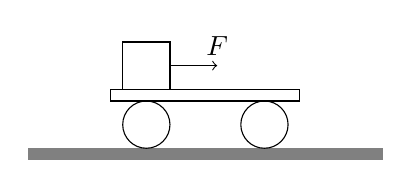
\begin{tikzpicture}[x=15mm,y=15mm]
	\draw(-1,0)--(2,0);
	\draw[draw=none,fill=gray](-1,0)rectangle(2,-.1);
	\draw(0,.2)circle(.2);
	\draw(1,.2)circle(.2);
	\draw(-.3,.4)rectangle(1.3,.5);
	\draw(-.2,.5)rectangle+(.4,.4);
	\draw[->](.2,.7)--+(.4,0)node[above]{$F$};
\end{tikzpicture}
\end{document}
